\chapter{Monitoring und Event Mgmt.}
\label{sec:monitoring}

\section{Sie kennen den Monitoring u. Event Management Prozess vertieft und können dessen wichtigsten Eigenschaften erläutern}

Überwachung der IT Services und erkennen der Fehlerzustände. 

\begin{itemize}
	\item Zeigt den Zustand aller Hardwaresysteme und Applikationen des gemonitorten IT Service an.
	\item Liefert Informationen zur präventiven Erkennungen möglicher Störungen.
	\item Konfiguriert Instrumente zur automatischen Überwachung, Steuerung von Systemen und zur Vermeidung von Störungen.
	\item Beinhaltet auch die automatische Behebung von Störungen mittels Scripts (Automation).
\end{itemize}

\begin{figure}[h!]
\centering
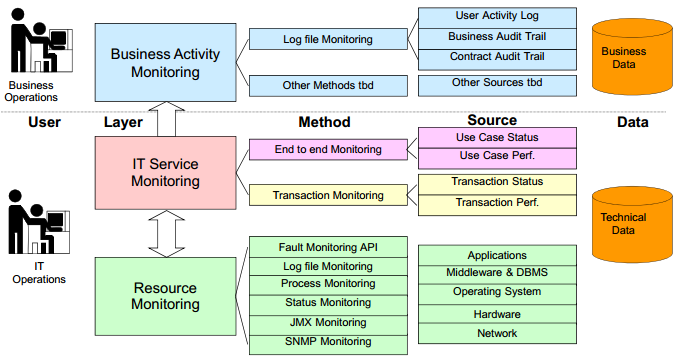
\includegraphics[width=0.7\linewidth]{fig/itil-monitoring-layers}
\caption{Monitoring Layers \& Technologies}
\label{fig:itil-monitoring-layers}
\end{figure}

\begin{description}
	\item[Monitored Object] Objekt das unter Beobachtung steht. Dies kann ein Prozess, eine Disk, die Memory, etc. sein.
	\item[Messpunkt] Pro monitored Object gibt es mind. 1 oder mehrere Messpunkte. Konkrete Charakteristika eines monitored object. Bsp: Füllgrad bei Disk, Lesezeit bei Disk.
\end{description}

\paragraph{Event-Management}
Bei einem Event handelt es sich um ein für die Services relevantes Ereignis. Eine in der unvorhergesehene Statusänderung eines oder mehrerer Configuration Items. Typischerweise ist dies eine Benachrichtigung, welches ein Service, ein Configuration Item oder ein Monitoring Tool generiert. Diese Events sind oft kategorisiert, bspw. Info, Warning, Exception. Im Event steht immer die Quelle und die Beschreibung des Zustandes.

Auf ein Event muss oft ein IT Mitarbeiter reagieren. 

Das Ziel im Event-Management ist es, diese Events zu entdecken, zu verstehen und angemessen zu handeln.

In grossen Infrastrukturen gibt es unzählige Events. Im Event-Management geht es auch darum, die wichtigen Events zu filtern, zu verknüpfen und anzureichern. Damit die IT Operatoren damit gut arbeiten können.

\section{Sie können die wichtigsten Funktionen eines Monitoring-Tools am Beispiel von NAGIOS erläutern}

NAGIOS ist OpenSource und bietet unzählige Monitoring Möglichkeiten. Windows, Linux/UNIX, Routers, Switches, Firewalls, Drucker, Services, Applikationen.

Benachrichtigungsmöglichkeiten über E-Mail, SMS und Web-Interface. Man kann Event-Handlers definieren - Reaktionen nach Problemerkennung - z.B. Neustart eines Webservers.

Reporting Options. SLA availability repots, alert and notifcation reports und weitere.

Multi-user, Skalierbar (bis zu 100 000 überwachende Nodes), bewährt, Failover protection, grosse Community.

\paragraph{Arten der Überwachung}
\begin{description}
	\item[Aktive Überwachung] Überprüfung wird durch Nagios initiiert.
	\item[Passive Überwachung] Überprüfung wird durch externe Programme initiiert. Antwort wird an Nagios gesendet und verarbeitet.
	\item[Direkte Überwachung] Nagios kann direkt, ohne Zwischenstellen, die Dienste prüfen. Öffentliche Dienste wie HTTP, FTP, Ping etc. auf lokalen und entfernten Rechnern. Lokale Dienste wie CPU load, disk usage etc. auf lokalen Rechnern.
	\item[Indirekte Überwachung] Nagios muss über Zwischenstellen wie der NRPE Agent, die Dienste überprüfen. Lokale Dienste auf entfernten Rechnern.
\end{description}

Nagios ist über Textdateien (cfg) konfigurierbar. timeperiods.cfg - Zeitangaben, wann überwacht werden soll. contacts.cfg - Kontakte, welche benachrichtig werden. commands.cfg - Überprüfungskommandos. localhost.cfg - überwachende Kommandos für den localhost. templates.cfg - Kommandos und Services können von Vorlagen erben.

Beispiel: Ich möchte die CPU Auslastung auf einem Rechner prüfen. Das ist eine indirekte Überwachung, da dies ein lokaler Dienst eines entfernten Rechners ist. Ich brauche den NRPE Agent check\_nrpe, CPU Load Pluging check\_load. 